% -----------------------------------------------
% LAMIR 2026 submission
% Timbre Morphing via Weight Interpolation of Specialized VAEs
% Double-blind (anonymized) version
% -----------------------------------------------

\documentclass{article}
\usepackage[T1]{fontenc} % add special characters (e.g., umlaute)
\usepackage[utf8]{inputenc} % set utf-8 as default input encoding
\usepackage{ismir,amsmath,cite,url}
\usepackage{graphicx}
\usepackage{color}
\usepackage{subcaption}

\usepackage{lineno}
\linenumbers

% Conference metadata for LAMIR 2026 (copyright notice / proceedings string).
\renewcommand{\conferenceyear}{2026}
\renewcommand{\conferenceedition}{2nd}
\renewcommand{\conferenceplace}{Belo Horizonte, Brazil}

% Relax float placement so wide (double-column) figures stay within the
% 4-page technical-content limit instead of being deferred.
\renewcommand{\topfraction}{0.92}
\renewcommand{\bottomfraction}{0.85}
\renewcommand{\textfraction}{0.06}
\renewcommand{\floatpagefraction}{0.7}
\renewcommand{\dbltopfraction}{0.92}
\renewcommand{\dblfloatpagefraction}{0.7}
\setcounter{topnumber}{3}
\setcounter{totalnumber}{5}
\setcounter{dbltopnumber}{3}

% Title (IEEE-compliant title case)
% ------
\title{Timbre Morphing via Weight Interpolation of Specialized Variational Autoencoders}

% Note: Please do NOT use \thanks or a \footnote in any of the author markup

% Anonymized submission: retain fake authors to preserve formatting.
\threeauthors
  {First Author} {Affiliation1 \\ {\tt author1@lamir.edu}}
  {Second Author} {\bf Retain these fake authors in\\\bf submission to preserve the formatting}
  {Third Author} {Affiliation3 \\ {\tt author3@lamir.edu}}

\def\authorname{F. Author, S. Author, and T. Author}

\sloppy % please retain sloppy command for improved formatting

\begin{document}

%
\maketitle
%
\begin{abstract}
Timbre morphing, the generation of intermediate timbres between known sounds,
expands the sonic palette for music production and sound design. Common
techniques interpolate in the latent space of a single generative model trained
on multiple timbres, which in small models compromises the fidelity of each one.
We propose an alternative: training variational autoencoders ($\beta$-VAE)
specialized per timbre, and generating hybrid timbres by interpolating directly
in the model weight space. The system is trained on STFT magnitude spectrograms
from four sources (piano, guitar, voice and bass) and evaluated with Fr\'echet
Audio Distance over MERT embeddings. Specializing each model by fine-tuning from
a common base model, rather than training it from scratch, yields more gradual
and predictable timbre transitions, especially when combined with latent-space
regularization ($\beta$-VAE). Being built on small, lightweight models, the
approach is potentially suitable for real-time synthesis.
\end{abstract}
%
\section{Introduction}\label{sec:introduction}

Timbre is the perceptual attribute that lets us distinguish two sounds of equal
pitch and loudness produced by different sources, such as the same note played
on a piano and on a guitar. Generating intermediate timbres between two known
sounds---commonly called timbre \emph{morphing}---is of particular interest for
music production and sound design: it enables exploring hybrid sonorities that
belong to no single source and thus expands the palette beyond traditional
timbres.

To synthesize such sonorities from familiar ones it is natural to draw on the
generative power of deep neural networks. The most widespread approaches learn a
single generative model over multiple timbres and interpolate within its latent
space; however, when the model is small this strategy tends to compromise the
fidelity of each individual timbre. This work explores an alternative: training
a specialized model per timbre and interpolating directly in the space of their
\emph{weights}, so as to preserve the reconstruction quality of each source
model when generating the intermediate states.

A design principle that runs through the whole proposal is to keep the models
deliberately small. We want them easy to train and to run, so that both
inference and the interpolation of their weights can be carried out with modest
hardware and, eventually, in real time. This orientation aims at a practical
tool for musical performance and production, and it conditions the architecture
and data decisions taken throughout.

\noindent\textbf{Contributions.} (i) We propose and validate a timbre-morphing
technique based on interpolating the \emph{weights} of per-instrument
specialized VAEs, instead of interpolating in the latent space as is usual in
the literature. (ii) We provide empirical evidence that two factors are
decisive for high-quality interpolations: latent-space regularization
($\beta$-VAE) and initializing the models from a common pre-trained checkpoint,
with regularization being the more impactful. (iii) We show that FAD combined
with MERT embeddings is a robust and consistent metric for timbre similarity,
outperforming cosine similarity in stability.

\section{Related Work}\label{sec:related}

Audio morphing can be organized by \emph{where} the interpolation that yields
the intermediate sound takes place: on the \textbf{signal}, on the
\textbf{latent space} of a generative model, or---as we propose---on the model
\textbf{weights}. A foundational signal-domain method \cite{slaney1996audiomorphing}
aligns two spectrograms with dynamic time warping and cross-fades them; it is
training-free but requires explicit alignment and was validated only on voice.
With deep learning, morphing moved to the latent space: NSynth
\cite{engel2017nsynth} interpolates note embeddings in a \emph{single}
WaveNet-decoder autoencoder trained on all instruments, materialized by Magenta
as an interactive grid \cite{magenta2017nsynthsoundmaker} close to the tool
motivating our work; its autoregressive decoder, however, precludes real-time
synthesis.

Recent work relies on latent diffusion, with high quality at high cost. Latent
diffusion bridges \cite{mancusi2025latentbridges} train one diffusion model per
instrument connected by a shared prior, but perform full timbre \emph{transfer}
rather than controllable intermediate states. SoundMorpher
\cite{niu2024soundmorpher} morphs in the noise and embedding space of a
pretrained text-to-audio model and introduces perceptually uniform morphing, at
the cost of a large model. For guitar tones, Chen \emph{et al.}
\cite{chen2025guitartonemorphing} find that a lightweight autoencoder beats
fine-tuned diffusion, and one variant interpolates network weights---the closest
contact point with our idea, though restricted to a single instrument.
Mix2Morph \cite{chu2026mix2morph} trains a large text-to-audio model to morph
from noisy mixes. Overall, the literature interpolates the \emph{content} inside
a fixed model; interpolating the \emph{parameterization} of distinct,
lightweight per-instrument models is the space this work occupies. We also adopt
FAD, on which the community has converged for timbre similarity.

Variational autoencoders (VAE) \cite{kingma2013auto} impose a probabilistic
structure on the latent space via the Kullback--Leibler (KL) divergence, which
facilitates sampling and interpolation; the $\beta$-VAE \cite{higgins2017beta}
weights this term by a scalar $\beta$ that balances reconstruction quality
against regularization. For music sound modeling, variational models offer the
best fidelity/regularization trade-off \cite{roche2019autoencodersmusicsoundmodeling};
RAVE \cite{caillon2021rave} showed real-time VAE synthesis; and sparse
autoencoders build perceptually consistent timbre spaces \cite{riera2017timbre}.

\section{Method}\label{sec:method}

\subsection{Dataset}
We work with four instruments: piano, guitar, bass and voice. They are familiar
and easily recognizable sources with clearly distinguishable timbres, a
necessary condition for evaluating timbre transitions. We gathered
approximately 87 minutes of real recordings per instrument (about 5.8 hours in
total), keeping the amount balanced to avoid biasing training. Piano was
collected from public-domain classical recordings; guitar from a subset of
GuitarSet \cite{xi2019guitarset} (electric guitar, melodic and chordal
passages); bass from jazz-standard basslines in FiloBass
\cite{riley2023filobass}; and voice from a representative subset of VocalSet
\cite{wilkins2018vocalset} (two male and two female voices, with melodies,
scales and arpeggios).

\subsection{Audio Representation and Preprocessing}
All tracks are converted to mono and resampled to $22050$~Hz. We then apply the
Short-Time Fourier Transform (STFT) with a $2048$-sample Hann window and a
$512$-sample hop, keeping magnitude and phase separately. Since timbral
information resides mainly in the spectral energy distribution, the model works
only with the magnitude, expressed in decibels as $S = 10\log_{10}(|F|^2)$,
where $F$ is the complex spectrum. We clip values below $-60$~dB, shift the
energy floor to zero, and divide by the global maximum $X_{max}$ (stored with
the model) to map magnitudes to $[0,1]$. Each spectrogram frame is thus a
$1025$-dimensional vector ($\textit{win\_length}/2 + 1$ bins), the unit fed to
the network; frames are processed independently, without explicitly modeling
their temporal evolution.

\subsection{Variational Autoencoder}
The VAE is a latent-variable generative model that assumes data are generated
from a latent variable $z$ with prior $p(z)=\mathcal{N}(0,I)$. The decoder
models the likelihood $p(x\mid z)$ and the encoder the approximate posterior
$q(z\mid x)$. Training maximizes the Evidence Lower Bound (ELBO), i.e.\
minimizes a reconstruction term plus a KL regularizer. The $\beta$-VAE
\cite{higgins2017beta} weights the KL term by $\beta$:
\begin{equation}\label{eq:loss}
\mathcal{L} = \mathcal{L}_{\mathrm{rec}} + \beta\,\mathcal{L}_{\mathrm{KL}},
\end{equation}
where under a Gaussian likelihood $\mathcal{L}_{\mathrm{rec}}$ reduces to the
mean squared error (MSE) between input and reconstruction, and
$\mathcal{L}_{\mathrm{KL}}$ is the closed-form KL divergence between $q(z\mid
x)$ and $\mathcal{N}(0,I)$. The latent vector is obtained via the
reparameterization trick $z = \mu + \varepsilon\odot\exp(\tfrac{1}{2}\log
\sigma^2)$, $\varepsilon\sim\mathcal{N}(0,I)$; when $\beta=0$ the KL term
vanishes, the model reduces to a deterministic autoencoder (AE) and we take
$z=\mu$. Higher $\beta$ pushes the posteriors toward the prior, yielding a
smoother, more continuous latent space at the cost of reconstruction fidelity.

\subsection{Architecture}
The encoder is a stack of fully connected layers that progressively reduce
dimensionality from the $1025$ input values down to the latent space, following
$1025\!\rightarrow\!(512,256,128,64,32,16,8)\!\rightarrow\!4$; each hidden layer
combines a linear transformation, Batch Normalization and an ELU activation.
The variational encoder outputs a mean vector $\mu$ and a log-variance vector
$\log\sigma^2$. The decoder mirrors this structure, expanding $z$ back to a
$1025$-dimensional magnitude spectrum; its final layer is linear (no
activation) so as not to restrict the reconstructed range. We use a latent
dimension of $4$ in most experiments, a choice justified empirically in
Section~\ref{sec:results}.

\subsection{Training Strategy}
We optimize Eq.~\eqref{eq:loss} with Adam (learning rate $10^{-3}$), a $95/5$
train/validation split, batches of $256$ frames, early stopping on the
validation loss and gradient clipping. Per-instrument models are obtained under
two initialization strategies. \emph{Scratch}: each model is trained from a
random initialization on its instrument only. \emph{Checkpoint}: we first train
a \emph{base model} on all four instruments to learn a general timbral
representation, and then fine-tune one model per instrument from that common
starting point. Combining the two initializations with two regularization
settings---AE ($\beta=0$) and $\beta$-VAE ($\beta=0.001$)---yields four
configurations per instrument that we compare in the experiments.

\subsection{Weight Interpolation}
Given two models with identical architecture, a source A and a target B, and a
coefficient $\alpha\in[0,1]$, we build an intermediate model whose parameters
combine those of A and B, parameter by parameter. By construction $\alpha=0$
reproduces A and $\alpha=1$ reproduces B, while intermediate values yield
decoders that synthesize mixed timbres. We explore linear interpolation (LERP),
$(1-\alpha)\,w_A + \alpha\,w_B$, and spherical interpolation (SLERP), which
traverses the arc joining both weight vectors:
\begin{equation}\label{eq:slerp}
\mathrm{SLERP}(w_A,w_B,\alpha)=
\frac{\sin\!\big((1-\alpha)\theta\big)}{\sin\theta}\,w_A +
\frac{\sin\!\big(\alpha\theta\big)}{\sin\theta}\,w_B,
\end{equation}
where $\theta$ is the angle between $w_A$ and $w_B$. When the vectors are nearly
parallel, SLERP becomes numerically unstable and we fall back to LERP.
Non-floating-point parameters (e.g.\ Batch Normalization counters) are not
interpolated: we take the value of the closer model according to $\alpha$.

\subsection{Audio Reconstruction and Metrics}
The decoder produces only a normalized magnitude spectrogram, which we rescale
by $X_{max}$ and invert to linear magnitude. Since the inverse STFT also needs
phase, we evaluate Griffin--Lim, PGHI \cite{prusa2017pghi} (a non-iterative,
single-pass phase-gradient method) and random phase, and apply the inverse STFT
with the analysis window. For evaluation we use: (i) reconstruction MSE on
validation, to compare latent sizes and $\beta$ values; (ii) Fr\'echet Audio
Distance (FAD) \cite{gui2024adaptingfrechetaudiodistance} over embeddings from
the pretrained MERT model \cite{li2023mert} (MERT-v1-95M), turned into a bounded
similarity $\mathrm{sim}=\exp(-\mathrm{FAD}/k)$; (iii) cosine similarity between
mean MERT embeddings, as an alternative baseline; and (iv) UMAP projections of
the latent embeddings, with a multidimensional Wilcoxon--Mann--Whitney $U$
statistic ($0.5$ = indistinguishable, $1$ = fully separated) to quantify
cluster separation per instrument pair.

\section{Experiments and Results}\label{sec:results}

\begin{figure*}[t]
\centering
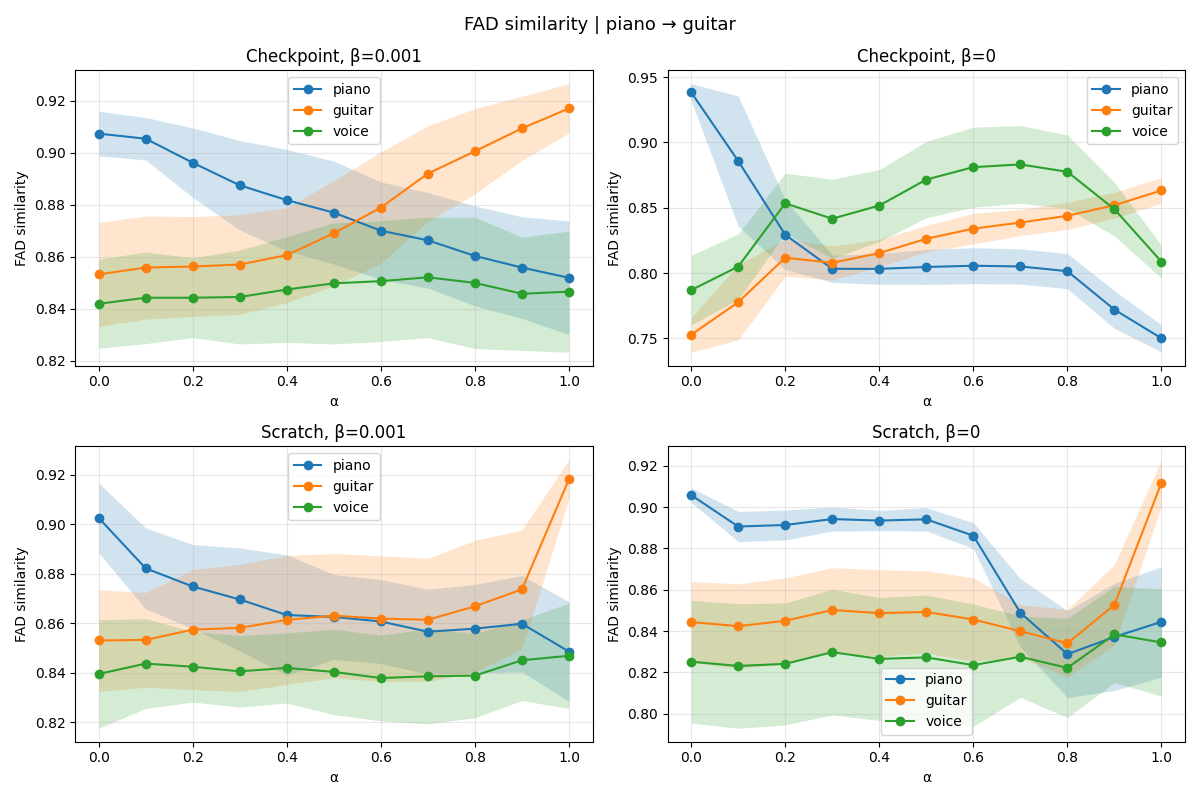
\includegraphics[width=0.88\textwidth]{figs/cross_transition.png}
\caption{Cross interpolation from piano (source A) to guitar (target B) with
voice as a witness instrument, for the four training configurations: FAD
similarity to each of the three instruments as the interpolation coefficient
$\alpha$ sweeps from $0$ to $1$. Only \emph{Checkpoint-$\beta$-VAE} (top left)
exhibits the expected behaviour---piano decreasing, guitar increasing, a
crossover near $\alpha=0.5$ and a flat witness. \emph{Checkpoint-AE} (top right)
transfers abruptly and perturbs the witness, while the \emph{Scratch} models
(bottom) barely change until $\alpha$ approaches $1$.}
\label{fig:cross}
\end{figure*}

\subsection{Architecture Exploration}
We first fix the latent dimension. Larger latent spaces reduce reconstruction
error, but for practical manipulation a small size is desirable (e.g.\ four
control knobs are more intuitive than thirty-two). Sweeping dimensions
$\{2,3,4,6,8\}$ and measuring the validation reconstruction error, a dimension
of $4$ gives a significant gain over $2$ and $3$, while $6$ or $8$ add little in
return; the same trend
holds for the $\beta$-VAE reconstruction error, for the KL divergence, and
consistently across all per-instrument models and the base model. We therefore
adopt latent dimension $4$.

Next we select $\beta$. Sweeping $\beta\in\{0,10^{-5},10^{-4},10^{-3},
10^{-2}\}$, we examine the trade-off between the mean reconstruction MSE and the
mean KL divergence on validation. Increasing regularization to $\beta=0.01$
excessively penalizes fidelity, whereas relaxing it to $10^{-4}$ or $10^{-5}$
inflates the KL divergence toward the unregularized ($\beta=0$) behavior without
a substantial reconstruction gain. The elbow of the curve sits at
$\beta=0.001$, which we adopt; informal listening confirmed that reconstructions
at $\beta=0.001$ are very close to those at $\beta=0$.

\subsection{Latent-Space Analysis}
Projecting the base-model latent embeddings to two dimensions with UMAP
($n\_neighbors=15$) and labeling each point by instrument, the four instruments
form clearly separated clusters under both $\beta=0$ and $\beta=0.001$, with
pairwise Wilcoxon--Mann--Whitney $U$ values close to $1$. Separation is
consistently slightly lower with $\beta=0.001$, consistent with regularization
producing a smoother, more continuous latent space (e.g.\ for the bass--voice
pair the statistic drops from $0.926$ at $\beta=0$ to $0.796$ at $\beta=0.001$).

\subsection{Choice of Similarity Metric}
We compare cosine similarity and FAD on a voice-to-piano interpolation, using
the piano reconstruction as reference and two ways of feeding the decoder: a
fixed random latent $Z$ (constant timbre) and a $Z$ obtained by encoding a real
validation clip (a trajectory through latent space). FAD stays stable and traces
smooth, low-variance transition curves in both cases and across configurations,
whereas cosine similarity, although it captures the general trend, is erratic
along latent trajectories (spurious peaks and drops, higher dispersion). Being
more robust and consistent, FAD is used for the rest of the analysis.

\subsection{Weight-Interpolation Experiments}
We first evaluate whether the timbre transfer holds regardless of the source and
target instruments, measuring FAD similarity as a function of $\alpha$ for the
four training configurations, averaged over many latent samples and over every
source/target instrument pair. Timbre transfer occurs in all four, but their
quality differs markedly. \emph{Checkpoint-$\beta$-VAE} ($\beta=0.001$) produces
the smoothest and most sustained growth in similarity towards the target and is
consistently the best configuration, followed by \emph{Scratch-$\beta$-VAE};
\emph{Scratch-AE} ($\beta=0$) is the worst, failing to transition gradually and
delaying the timbre change to extreme values of $\alpha$. This indicates that the
regularization imposed by $\beta>0$ is the factor with the greatest impact on
interpolation quality, while sharing a common weight initialization
(\emph{Checkpoint}) contributes a further improvement. Both the per-source
breakdown and the aggregation over all source/target combinations reproduce this
ordering, so it is not an artifact of a particular instrument pair.

A stricter test of the method is the cross-interpolation property: as the
synthesized audio approaches target B it must move away from source A while
\emph{not} acquiring traits of an unrelated \emph{witness} instrument that takes
no part in the interpolation. Figure~\ref{fig:cross} reports this experiment with
A = piano, B = guitar and voice as witness, tracking the FAD similarity to the
three instruments as $\alpha$ sweeps from $0$ to $1$ under each configuration.
The expected behaviour---similarity to A decreasing, similarity to B increasing,
both curves crossing near $\alpha=0.5$, and the witness remaining flat---is met
only by \emph{Checkpoint-$\beta$-VAE}. The \emph{Scratch} models depart from it
precisely in the intermediate range that matters for morphing: with
$\beta=0.001$ the transfer is inconsistent, and with $\beta=0$ it is practically
nonexistent until $\alpha>0.8$, meaning the intermediate models remain locked to
the source timbre instead of synthesizing hybrids. \emph{Checkpoint-AE} does
achieve the transfer, but abruptly and with erratic fluctuations in the witness
curve, indicating that its intermediate decoders drift towards timbres unrelated
to either endpoint. These results confirm that a common initialization combined
with a regularized latent space (\emph{Checkpoint} with $\beta=0.001$) is what
yields a predictable, gradual and independent timbre transfer.

\subsection{Audio Examples}
To complement the quantitative analysis with a perceptual assessment, audio
examples of continuous timbre transitions (voice-to-piano and guitar-to-piano,
using the \emph{Checkpoint-$\beta$-VAE} configuration) and of audio-to-audio
morphing between real recordings are provided as supplementary material.

\section{Conclusions}\label{sec:conclusions}

We developed and validated a technique to synthesize intermediate timbres
between instruments by interpolating the weights of specialized VAE models.
Unlike conventional techniques that operate within the latent space of a single
model trained on multiple instruments, our approach trains an independent model
per instrument and interpolates directly over its parameterization, producing
intermediate decoders that generate hybrid timbres. A latent dimension of $4$
offers the best trade-off between reconstruction fidelity and manipulability,
and $\beta=0.001$ sits at the elbow of the reconstruction--KL curve. The central
finding is that interpolation quality depends strongly on the training
configuration: regularizing the latent space ($\beta$-VAE) and starting from a
common base model via fine-tuning (\emph{Checkpoint-$\beta$-VAE}) consistently
produced the smoothest and most predictable transitions, both in the FAD metric
and in subjective listening. FAD over MERT embeddings proved a robust similarity
metric, outperforming cosine similarity in stability.

A deliberate design choice was to work with small models and a limited amount of
data (about 87 minutes per instrument, four instruments), so as to keep the
models easy to train, lightweight and runnable on modest hardware---aligned with
the goal of a future real-time synthesis tool. As a counterpart, this limits the
attainable fidelity and generality; we view it as a conscious balance between
quality and lightweight, real-time viability rather than an intrinsic limitation
of the method. Future work includes real-time inference and weight
interpolation, integration into audio-production tools (e.g.\ VST plugins),
enlarging the dataset and instrument set, and extending the technique to a
triple interpolation controlled by two parameters.

\section{Ethics Statement}

This work uses publicly available datasets (GuitarSet, FiloBass, VocalSet) under
their respective licenses, together with public-domain piano recordings, and
does not involve the collection of personal or private data. The proposed
generative technique is intended as a creative tool for music production and
performance; as with any audio-synthesis method, care should be taken to respect
the rights of performers whose recordings are used to train the models.

% For bibtex users:
\bibliography{references}

\end{document}
